% Homework 13.tex 

\documentclass{article}
\usepackage{graphicx} % for figures
\usepackage{float}
\usepackage[export]{adjustbox}
\usepackage{fancyhdr}
\begin{document}

\title{Homework 11 - Physics 240\\
		System of Spring and Matrix Inversion}
\author{Tin Tran}

\maketitle

\section{Introduction}
Similar to the previous homework, this is a continuation with polynomial fitting for the data. With the same set of mock data, now I apply polynomial fitting and I got this plot.
\begin{figure}[H]
\centering{
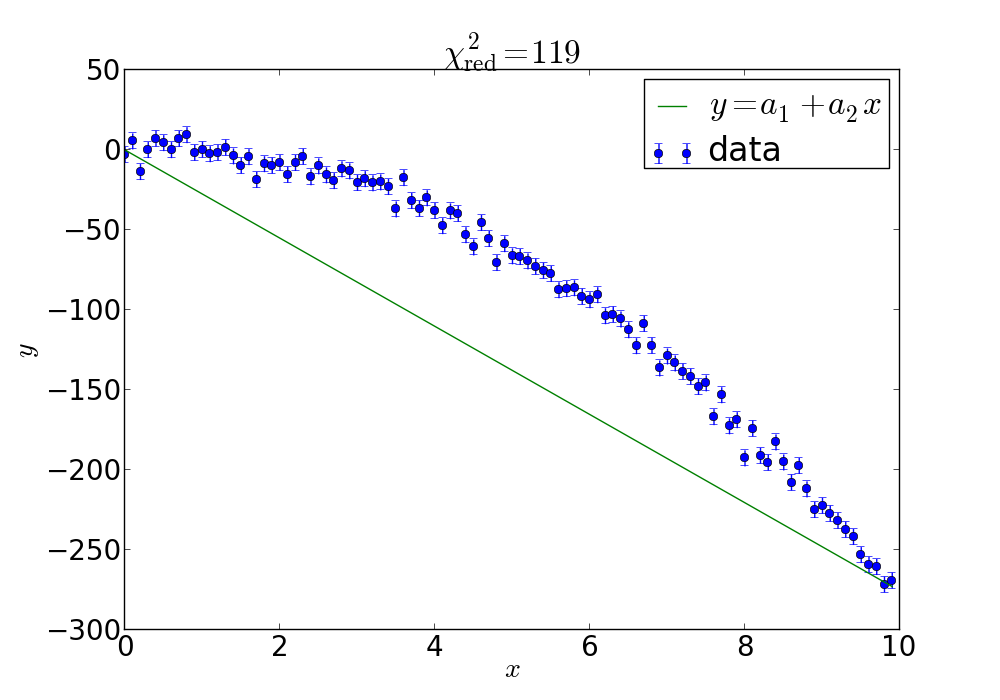
\includegraphics[max size={\textwidth}{\textheight}]{hw14a.png}
\caption{Polynomial fit with 2 paramaters}
}
\end{figure}
The $\chi ^2 _{red}$ value is not the same as with the linear fit, this could be because the mock data set is different for the polynomial fit. Other than that I have no other explaination.\\
With the 3 parameters, I get the following plot.
\begin{figure}[H]
\centering{
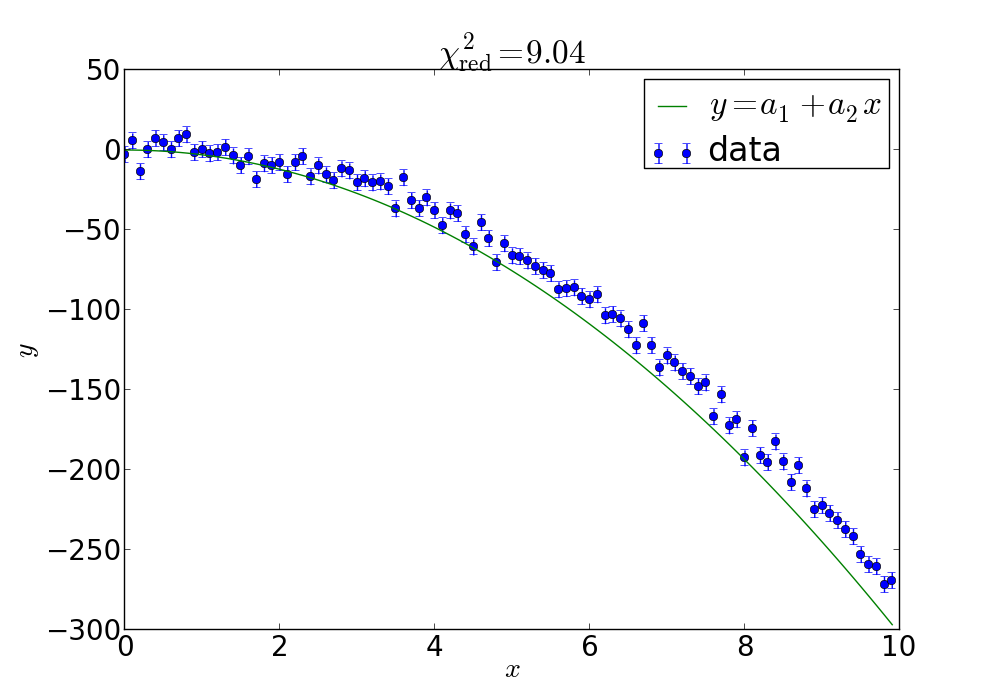
\includegraphics[max size={\textwidth}{\textheight}]{hw14b.png}
\caption{Power-law fit of Global Temperature vs time}
}
\end{figure}
This shows that the code works for the mock data set with 3 parameters.
\section{Discussion and data}
I got my data from NASA giss, specifically the Global annual mean surface air temperature change vs time. After fitting the data, I got the following outputs
\begin{figure}[H]
\centering{
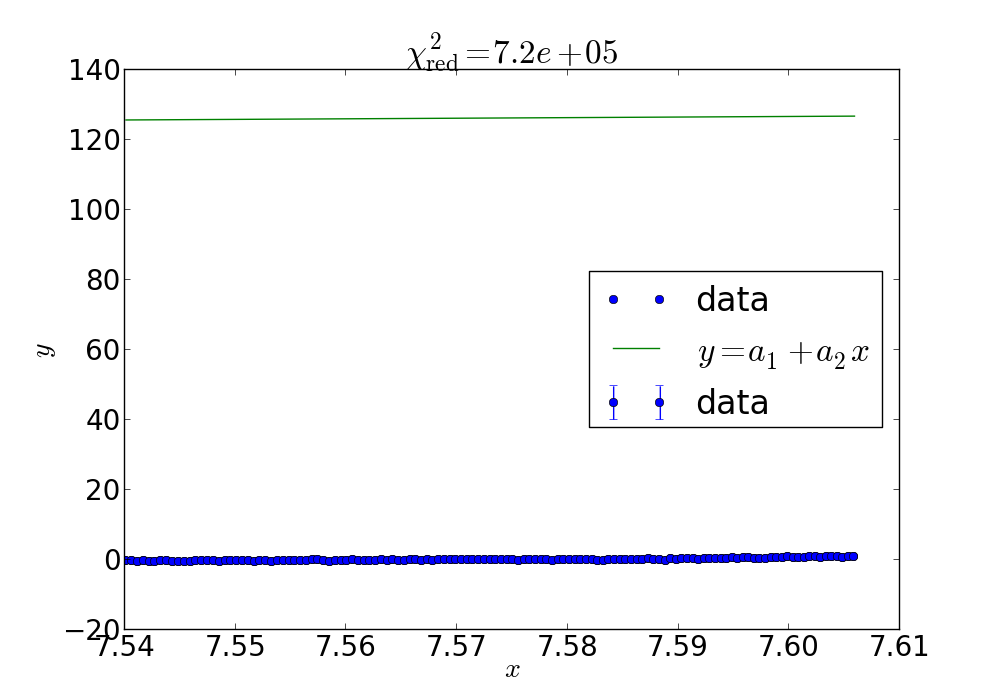
\includegraphics[max size={\textwidth}{\textheight}]{hw14c.png}
\caption{Polynomial fit of Global Temperature vs time 2 parameters}
}
\end{figure}
This is to test the polynomial fit with my data for 2 parameters, and I have no idea why my data can't get a good fit with polynomial, all the numbers seem to be very high. I'm guessing it's because the data is less than 1 and some are negative. The 3 parameters fit also gives a similar plot with no improvements.

\begin{figure}[H]
\centering{
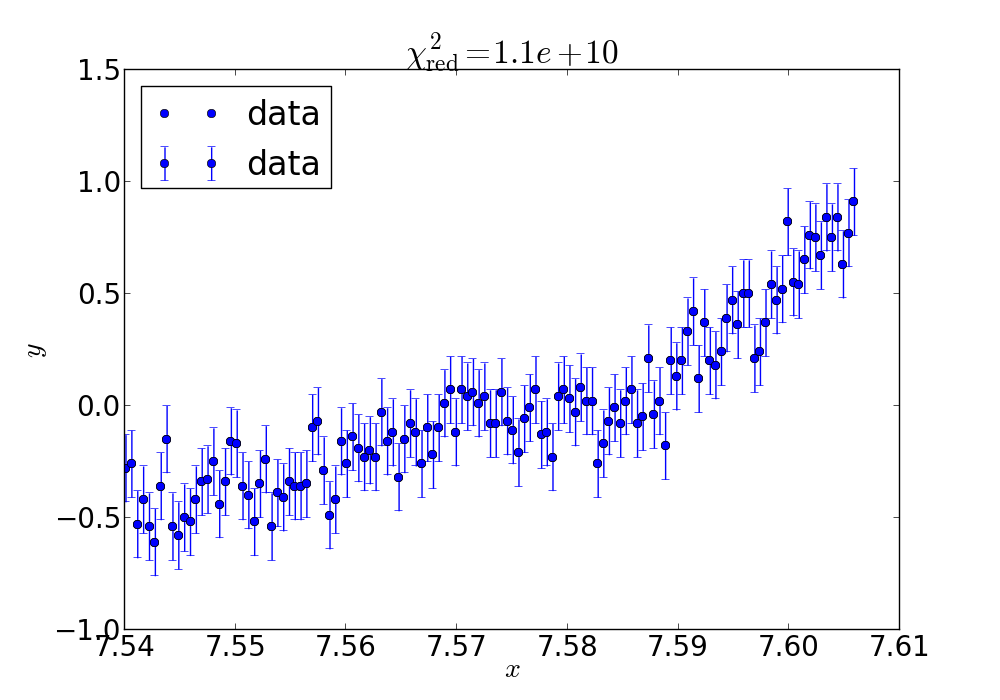
\includegraphics[max size={\textwidth}{\textheight}]{hw14d.png}
\caption{Global Temperature vs time}
}
\end{figure}
This is the data set that I got, and I reckon the polynomial should have no trouble fitting this set, but then I'm not sure why the fit works for the mock data and not my data set.

* I didn't have time to complete the contour plot because I into some trouble with the array.
\end{document}